%% Template for SDP report, adapted from mlp_cw2_template, 2018. 

%% Based on  LaTeX template for ICML 2017 - example_paper.tex at 
%%  https://2017.icml.cc/Conferences/2017/StyleAuthorInstructions

\documentclass{article}
\usepackage[T1]{fontenc}
\usepackage{amssymb,amsmath}
\usepackage{txfonts}
\usepackage{microtype}
\usepackage{xspace}
\xspaceaddexceptions{\%}

% Lists with less spacing between items
\usepackage{paralist}

% For figures
\usepackage{graphicx}
\usepackage{subfig} 

% For citations
\usepackage{natbib}

% For algorithms
\usepackage{algorithm}
\usepackage{algorithmic}

% the hyperref package is used to produce hyperlinks in the
% resulting PDF.  If this breaks your system, please commend out the
% following usepackage line and replace \usepackage{mlp2017} with
% \usepackage[nohyperref]{mlp2017} below.
\usepackage{hyperref}
\usepackage{url}
\urlstyle{same}

% Packages hyperref and algorithmic misbehave sometimes.  We can fix
% this with the following command.
\newcommand{\theHalgorithm}{\arabic{algorithm}}


% Set up MLP coursework style (based on ICML style)
\usepackage{mlp2018}
\mlptitlerunning{SDP Demo \demoNumber  Group (\groupNumber)}
\bibliographystyle{icml2017}


\DeclareMathOperator{\softmax}{softmax}
\DeclareMathOperator{\sigmoid}{sigmoid}
\DeclareMathOperator{\sgn}{sgn}
\DeclareMathOperator{\relu}{relu}
\DeclareMathOperator{\lrelu}{lrelu}
\DeclareMathOperator{\elu}{elu}
\DeclareMathOperator{\selu}{selu}
\DeclareMathOperator{\maxout}{maxout}







%% You probably do not need to change anything above this comment

%% REPLACE the details in the following commands with your details
\setGroupNumber{20}
\setGroupName{ENRS}
\setProductName{FInDO}
\setLogoFileName{figs/sdp_logo_placeholder.png}

\begin{document} 

\makeSDPTitle{Project Plan}

% Previous MLP Style Title Layout working. 
% \twocolumn[
    % \mlptitle{\productName: SDP Demo \demoNumber}
    % \centerline{Group \groupNumber: \groupName}
% ]

\begin{abstract} 
The abstract should first consist of one sentence describing the intended functionality of your system. It should be followed by a few sentences (100--200 words) summarising the main milestones that will bring your project to a successful completion. This should give the reader a clear expectation of what will be achieved throughout the semester.
\end{abstract} 


\section{Goal description} 
This section should start with a paragraph stating, in simple words, the key idea of your system. Describe the problem in one sentence, and use another sentence to describe your solution.

\subsection{Relevance of the system} 
If possible you should then provide evidence that the problem is relevant, by referencing published research that demonstrates a need and / or characterizes a potential market for your system. If appropriate, include reference to existing systems that you are taking as inspiration. You should cite the sources (e.g. \cite{Newell81}) and add the details to the example-refs.bib file so that the full references appears in the bibliography section.

\subsection{High-level description} 
You should then provide the description of your problem in terms of functionalities. A common approach in the software industry is to rely on user stories. Internet is full on resources on the topic and you should investigate it.


\section{Task planning}
In this section you must provide a detailed plan of the tasks to be completed to achieve your goals. The plan must comprise two levels: first a few milestones that correspond to major achievements in the project, then a detailed list of atomic tasks that must be achieved.

\subsection{Milestones} 
From the user stories, you should extract the main technical subgoals, i.e., what you need to accomplish to get to the desired final result. For each subgoal you should provide an explicit milestone that states what you should have achieved, by what date, and what evidence you will present to show you have achieved it (e.g. a demonstration of the feature to the experts).


\subsection{Task decomposition} 
Each milestone should then be decomposed into a set of ``atomic'' tasks, taking no more than 20 hours each. Each task should be given a name, a one-sentence-long description, and an estimated time for completion.


You can summarize the tasks in a table, (for instance, table~\ref{tab:sample-table}, using the \verb+table+ environment).

\begin{table*}[h]
\vskip 3mm
\begin{center}
\begin{small}
\begin{sc}
\begin{tabular}{lcccr}
\hline
\abovespace\belowspace
Task Name & Milestone  & Estimated time & Dependency &  Rough description \\
\hline
\abovespace
Task 1 & Milestone 1    & 0.5 Days & - & Description 1 \\
Task 2 & Milestone 1    & 1 Day  & Task 1 & Description 2 \\
Task 3 & Milestone 2    & 2 Days & Milestone 1 & Description 3 
\belowspace
\end{tabular}
\end{sc}
\end{small}
\caption{Task decomposition for the system}
\label{tab:sample-table}
\end{center}
\vskip -3mm
\end{table*}

The report must include a Gantt chart, which should clearly identify any dependencies between the tasks. You may find it useful to make a revised version of your plan/gantt chart at key points in the project, in discussion with the experts. 

You can include the Gantt chart as a Latex figure (such as figure~\ref{fig:sample-fig}), use the \verb+\includegraphics+ environment to include an image (pdf, png, or jpg formats), ideally with informative labels added. 

To keep your folders clean, it is often a good idea to keep your images in a separate folder. In this example, we've put the figures in the \texttt{figs/} folder. To include images from different folders, give the relative path from this file. Example: \verb+\includegraphics{figs/image_filename}+.

\begin{figure}[tb]
\vskip 5mm
\begin{center}
\centerline{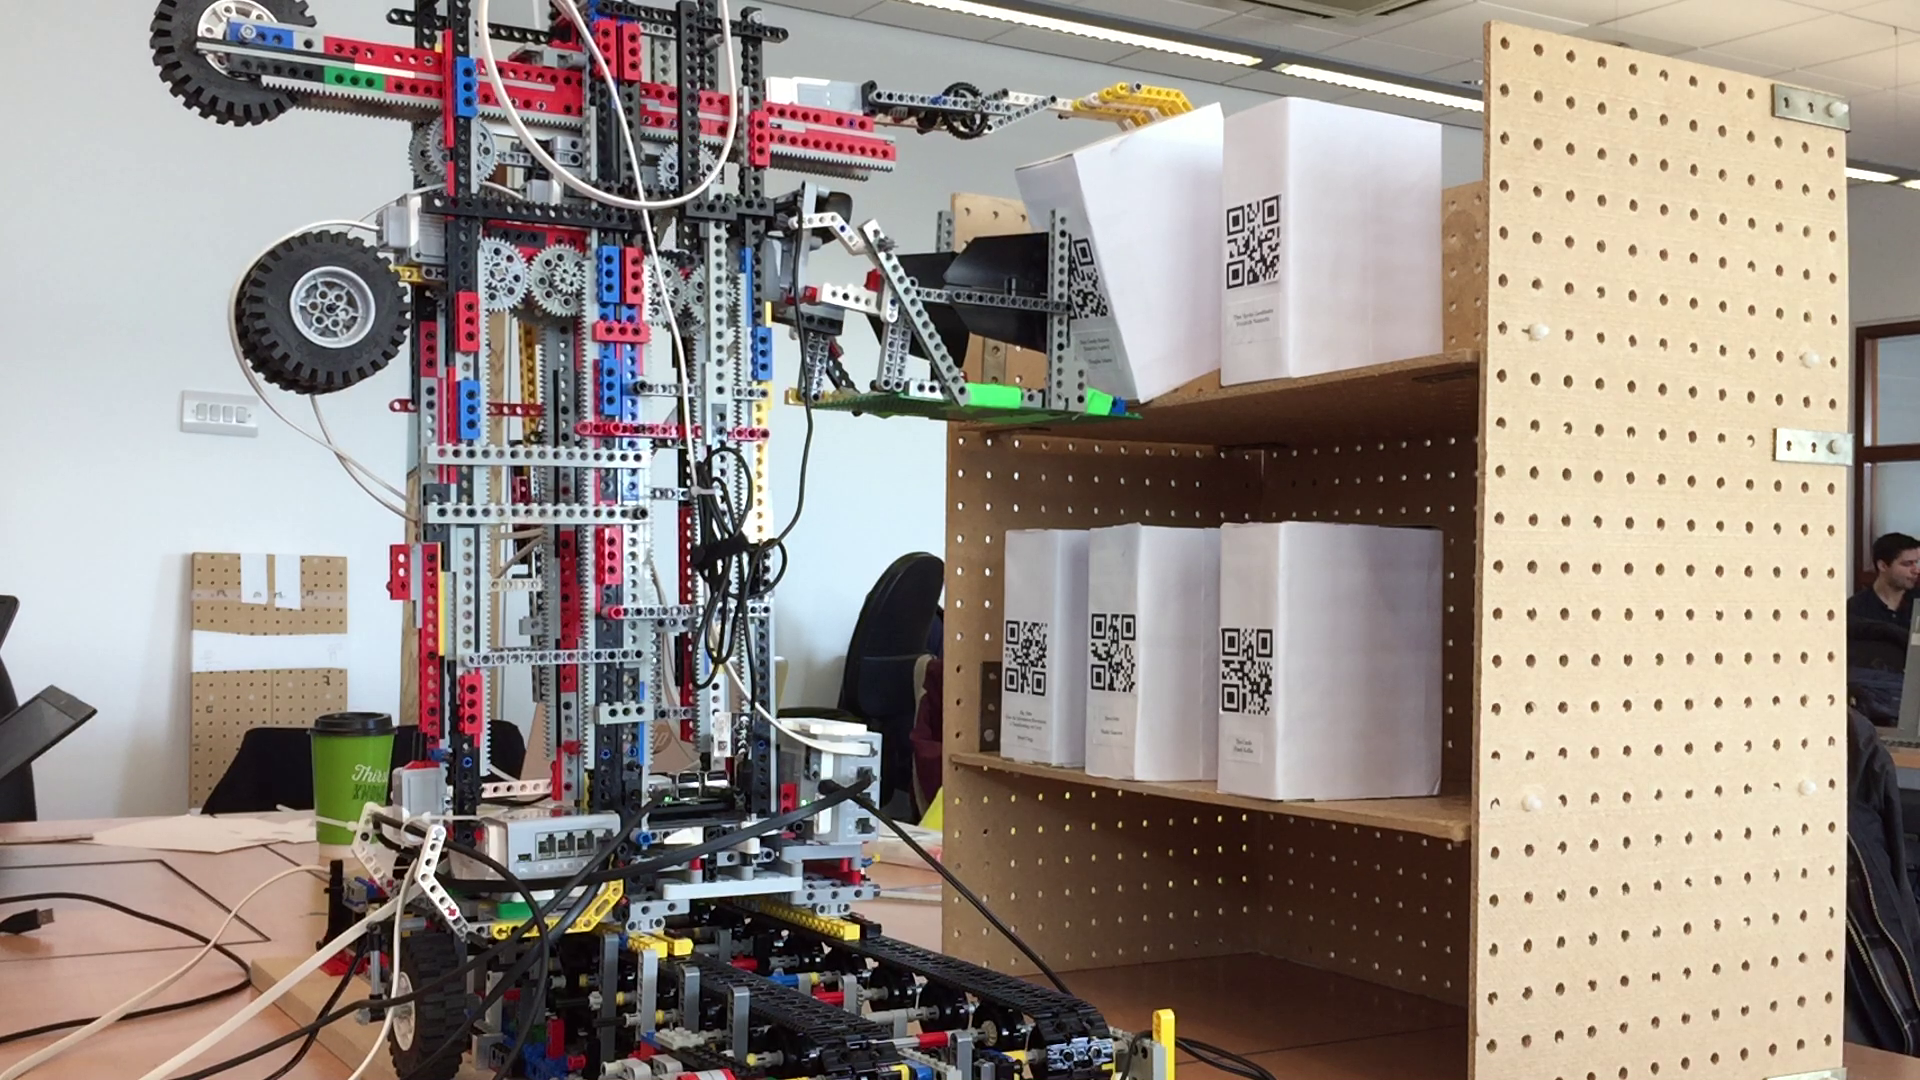
\includegraphics[width=\columnwidth]{figs/crane}}
\caption{Lego construction: highlight any salient features in the caption}
\label{fig:sample-fig}
\end{center}
\vskip -5mm
\end{figure} 


\subsection{Resource distribution}
The plan should explain how you will deploy your resources - 200 hours per group member over the semester - to achieve your goals. Note you should take into account time required by scheduled sessions (workshops, demo days, final presentations) and time used in planning and presenting (group meetings, report writing etc.). 

You should also list the resources you have in terms of skills, equipment, etc. The use of tables is also recommended for this section.

\subsection{Risk assessment} 
The report should also contain an assessment of the risks that you anticipate for the project, and contingency planning that you have done to guard against them. 

\section{Group organisation}
Finally, how you organise yourselves as a group and plan your work will be key to your success within the System Design project. You should detail the approach that you have taken to group organisation (e.g. specific roles of group members), meetings, communication, code-sharing, task allocation, and progress tracking.

%% Include any references in a bibliography

\bibliography{example-refs}

\end{document} 

